\documentclass[utf8,14pt]{beamer} % TODO remove handout for steps

% !TeX root = main.tex

\usepackage{graphicx}
\usepackage{amsmath}
\usepackage{tikz}
\usepackage[%
	backend=biber,
	url=false,
	style=numeric,
	maxnames=4,
	minnames=3,
	maxbibnames=99,
	giveninits,
	uniquename=init]{biblatex}
\usepackage{pgfpages}
\usepackage{multicol}
\usepackage{multirow}
\usepackage{appendixnumberbeamer}

\bibliography{bibliography}

\newcommand{\labelname}[1]{
	\def\insertenumlabel{#1}%
	\usebeamertemplate{enumerate item}%
}

\usefonttheme[onlymath]{serif} % use classic math font

\setcounter{secnumdepth}{1} % only sections for table of contents
\setcounter{tocdepth}{1}

\beamertemplatetransparentcoveredmedium
\beamertemplateballitem
\beamertemplatebookbibitems
\usenavigationsymbolstemplate{} % hide controls
\setbeamertemplate{footline}[frame number]
\usetheme{default} % plain white with blue headings

\setbeamertemplate{footline}
{
	\leavevmode%
	\hbox{%
		\begin{beamercolorbox}[wd=.333333\paperwidth,ht=2.25ex,dp=1ex,center]{author in head/foot}%
			\usebeamerfont{author in head/foot}\insertsection
		\end{beamercolorbox}%
		\begin{beamercolorbox}[wd=.333333\paperwidth,ht=2.25ex,dp=1ex,center]{title in head/foot}%
			\usebeamerfont{title in head/foot}\insertsubsection
		\end{beamercolorbox}%
		\begin{beamercolorbox}[wd=.333333\paperwidth,ht=2.25ex,dp=1ex,right]{date in head/foot}%
			\usebeamerfont{date in head/foot}\insertshortdate{}\hspace*{2em}
			\insertframenumber{} / \inserttotalframenumber\hspace*{2ex}
	\end{beamercolorbox}}%
	\vskip0pt%
}

\usefonttheme{structurebold}

\usecolortheme{rose} % orchid for a more dark version
\definecolor{orange}{rgb}{1,.549,0}
\definecolor{pink}{rgb}{1,0.5,0.5}
\definecolor{green}{rgb}{0,0.5,0}

% hide steps
\setbeamercovered{invisible}

% Tiny bib and add labels
\renewcommand*{\bibfont}{\scriptsize}
\setbeamertemplate{bibliography item}{\insertbiblabel}

\title{A Tool Architecture for the Continuous Detection of Open-Source License Infringements using Clone Detection}
\subtitle{{\small Masterarbeit}}
\author{Benedikt Schlagberger}
\institute[TUM]{{\small Technische Universität München}}
\date{05.02.2018}

\begin{document}
{
		\setbeamertemplate{footline}{} 
		\begin{frame}
			\titlepage
			\note{
				\begin{itemize}
					\item Halbes Jahr
					\item Entwicklung Werkzeug open source Lizenzverstößen aufdecken
					\item "Open source" verbindet man Wiederverwendung
					\item Lizenzverletzungen!
				\end{itemize}
			}
		\end{frame}
}

\begin{frame}
	\centering
	\begin{tikzpicture}[remember picture,overlay]
		\node[at=(current page.center)] {
			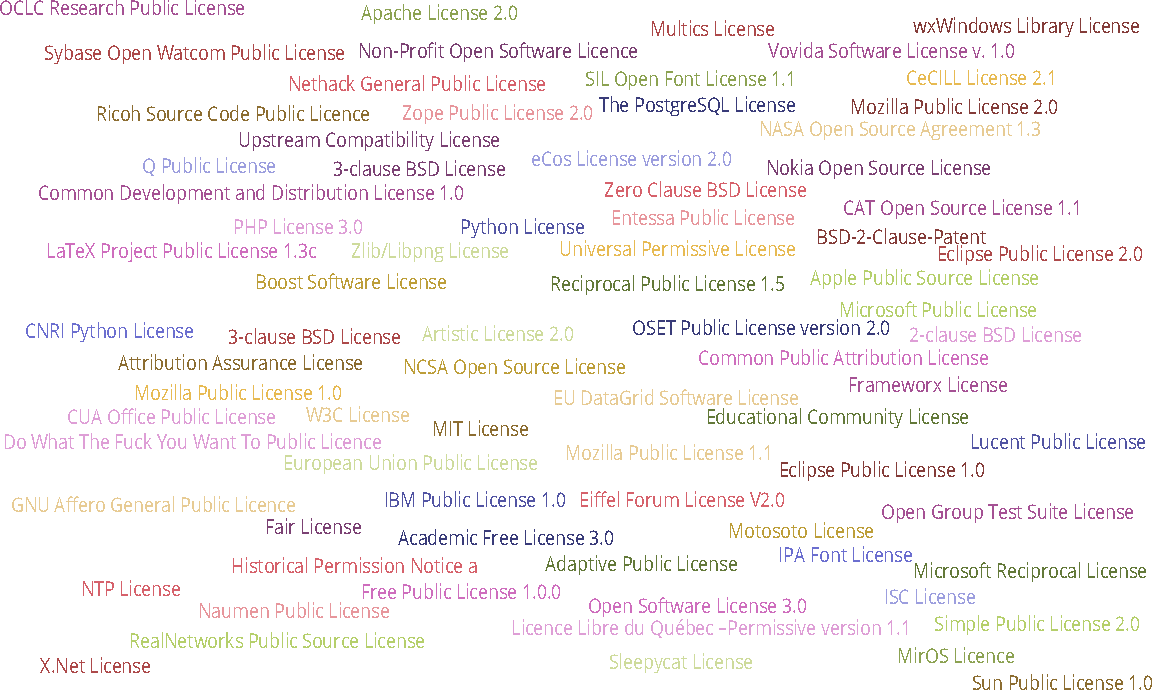
\includegraphics[width=0.9\paperwidth]{fig/wordcloud.pdf}
		};
	\end{tikzpicture}
	\note{
		\begin{itemize}
			\item Viele Open Source Lizenzen, kleiner Ausschnitt der Bekannteren
			\item anpassbar, selbst entwickeln
			\item Kompliziert, darf ich kopieren?
			\item JSON-License: "The Software shall be used for Good, not Evil"
			\item Tool: Kopieren erlaubt
		\end{itemize}
	}
	%TODO Oracle Binary Code License: I. SOURCE CODE. Software may contain source code that, unless expressly licensed for other purposes, is provided solely for reference purposes pursuant to the terms of this Agreement. Source code may not be redistributed unless expressly provided for in this Agreement.
\end{frame}

\frame{\frametitle{Outline} 
	\small
	\tableofcontents
	\note{
		\textbf{Aufbau der Arbeit:}
		\begin{itemize}
			\item Andere Arbeiten
			\item Daraus folgernd: Ansatz
			\item Analyse Performanz, kann Lizenzverletzungen aufdecken?
			\item Abschließend geb ich kurzes Fazit
		\end{itemize}
	}
}

% !TeX root = main.tex

\section{Related Work}
\begin{frame}{\insertsection}
	\begin{itemize}
	\normalsize
	\item Plagiarism detection in student submissions (\textit{YAP3, JPLAG, MOSS, dup, SID, GPLAG, ...})
	\item Clone detection for enhancing software quality (\textit{CCFinder, ConQat...})
	\item Code search engines (\textit{Sourcerer, SeCold, SeClone, ...})
	\item Commercial tools (\textit{Blackduck, Flexnet, ...})
	\end{itemize}
\end{frame}
% !TeX root = main.tex

\section{Approach}

\begin{frame}{\insertsection}
	\begin{itemize}
		\setlength{\itemsep}{8pt}
		\item \textit{Continuous detection} \onslide<2->\\
			$\rightarrow$ \textbf{Index-based approach}\onslide<3->
		\item \textit{High accuracy}\onslide<4->\\
			$\rightarrow$ \textbf{Indexing History}\onslide<5->
		\item \textit{Huge amount of open source code}\onslide<6->\\
			$\rightarrow$ \textbf{Server-client architecture}\onslide<7->
		\item \textit{Confidentiality}\onslide<8->\\
			$\rightarrow$ \textbf{Sending hashes instead of source code}\onslide<9->
		\item \textit{High number of lookup-requests}\onslide<10->\\
			$\rightarrow$ \textbf{Filtering hashes on client}
	\end{itemize}
\end{frame}

\subsection{Architecture}
\begin{frame}{\insertsubsection}
	\only<1>{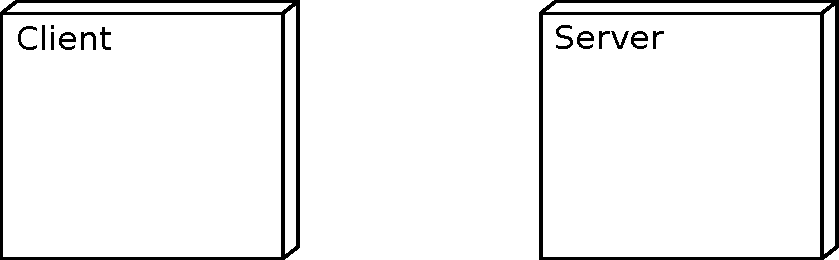
\includegraphics[width=\linewidth]{fig/architecture_overview_client_server.pdf}}
	\only<2>{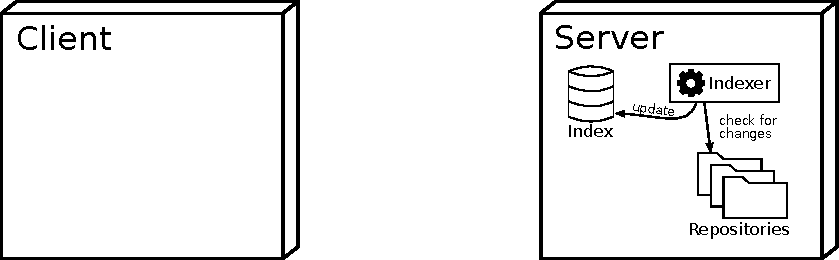
\includegraphics[width=\linewidth]{fig/architecture_overview_server.pdf}}
\end{frame}

\subsection{Index Creation}
\subsubsection{Normalization}
\begin{frame}{\insertsubsection}{\insertsubsubsection}
	\begin{center}
		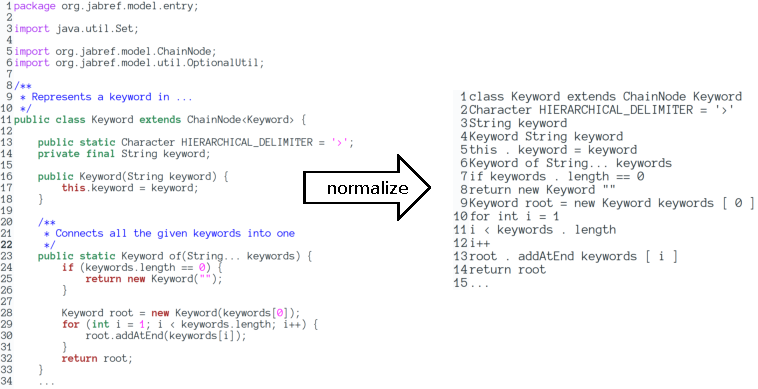
\includegraphics[width=0.9\linewidth]{fig/normalization_1.pdf}
	\end{center}
	\begin{itemize}
		\small
		\item Removes formatting, comments, access modifiers, brackets, import statements, ...
		\item Focus on features and properties relevant for comparing copied code
	\end{itemize}

	\note{
		\begin{itemize}
			\item Entfernt Formattierung, comments, access modifiers, brackets, import statements, keywords like final/static
			\item Übriges: "Fingerabdruck" (Struktur, Variablennamen, Literale, ...)
		\end{itemize}
	}
\end{frame}

\subsubsection{Hashing chunks}
\begin{frame}{\insertsubsection}{\insertsubsubsection}
	\begin{center}
		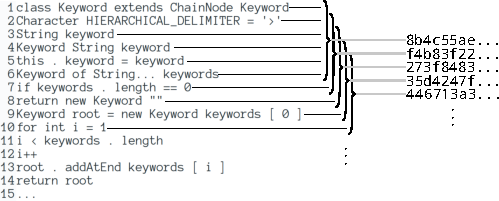
\includegraphics[width=0.9\linewidth]{fig/normalization_2.pdf}
	\end{center}
	\begin{itemize}
		\item Splitting normalized code into statements
		\item Group into chunks of 5 statements
		\item Location of chunk is stored in index
		\item Hash is used as key
	\end{itemize}
	\note{
		\begin{itemize}
			\item Index is key value store
		\end{itemize}
	}
\end{frame}

\subsubsection{History Analysis}
\begin{frame}{\insertsubsection}{\insertsubsubsection}
	\begin{center}
		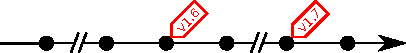
\includegraphics[width=\linewidth]{fig/history_analysis.pdf}
	\end{center}
	
	\begin{itemize}
		\item Analyzing history relevant to find old versions of a file
		\item Using git tags as reference points
		\item Re-indexing changed files between two versions
	\end{itemize}
\end{frame}

\begin{frame}{\insertsubsection}
\only<3>{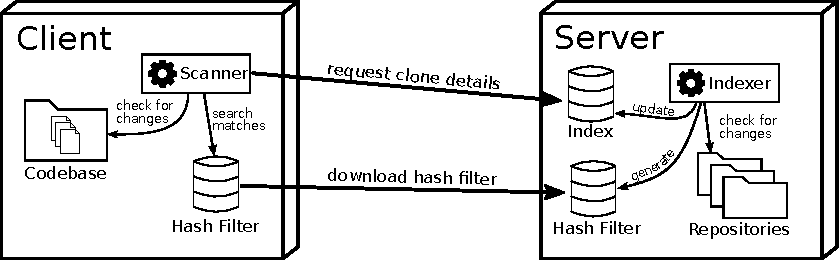
\includegraphics[width=\linewidth]{../written/figures/architecture_overview.pdf}
\begin{description}
	\small
	\item[Target System] System on client which should be scanned for copied code
	\item[Reference System] Open source software system on server
\end{description}
}
\note{
\begin{itemize}
	\item TODO
\end{itemize}
}
\end{frame}

\subsection{Searching for Copied Code}
\begin{frame}{\insertsubsection}
	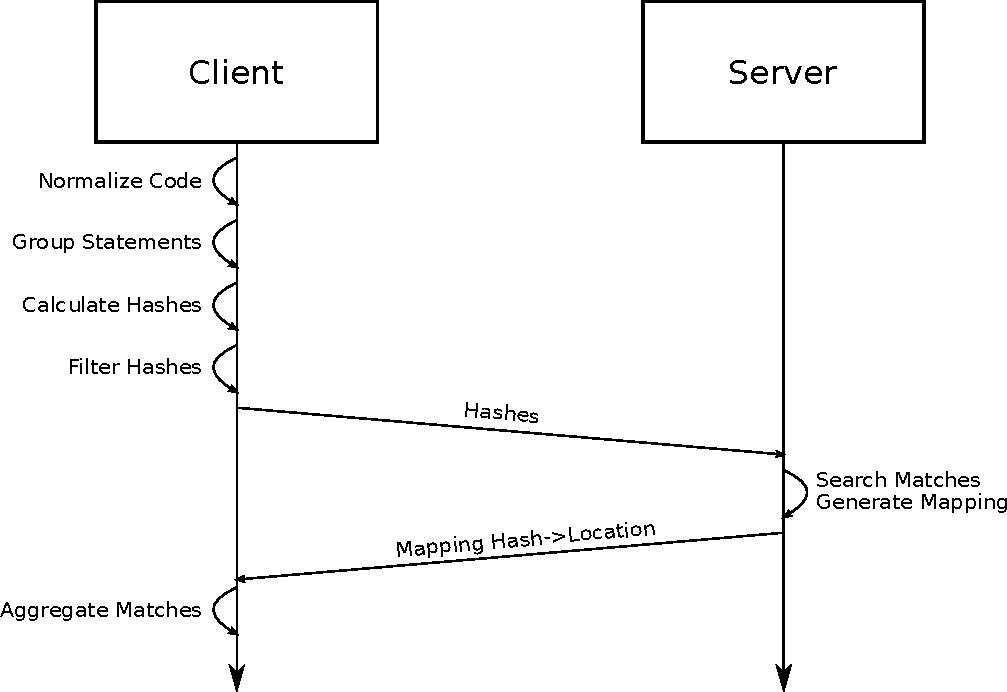
\includegraphics[width=\linewidth]{../written/figures/searching_copied_code.pdf}
\end{frame}

\subsubsection{Hash Filter}
\begin{frame}{\insertsubsection}{\insertsubsubsection}
\textbf{Problem:} Lots of request have to be sent to server\\
\pause
\vspace{2mm}
\textbf{Solution:} Bloom filter on client side
\vspace{2mm}
\begin{itemize}
	\small
	\item Data structure, calculated on server, downloaded to client
	\item Client can decide whether a hash is part of the index with very small false positive probability (0,01\%)
	\item Fraction in size compared to the index database\\ (37 GB $\rightarrow$ 200 MB)
	\item Reduces number of requests to a fraction
\end{itemize}
\end{frame}

%TODO aggregation?

% !TeX root = main.tex

\section{Evaluation}
\begin{frame}
	\frametitle{Outline} 
	\tableofcontents[
		currentsection,
		subsectionstyle=hide
	]
	
	\note{
		\begin{itemize}
			\item Ziel: Performanz des Ansatzes und Brauchbarkeit der Ergebnisse untersuchen
		\end{itemize}
	}
\end{frame}

\subsection{Step 1}
\begin{frame}{\insertsubsection}
	\textbf{Indexing 1000 Java and 1000 C/C++ GPL licensed projects from GitHub}
	
	\begin{table}[ht]
		\centering
		\scriptsize
		\begin{tabular}{l|rrrrr}
			& \textbf{Scanned Files} & \textbf{Lines of Code} & \textbf{Total size} & \textbf{Hashes} & \textbf{Chunks} \\ 
			\hline 
			Java & 836.555 & 57.834.764 & 94 GB & 23.773.065 & 35.069.633 \\
			C/C++ & 1.023.092 & 380.338.327 & 102 GB & 61.349.163 & 221.315.454 \\ 
		\end{tabular}
	\end{table}

	\begin{itemize}
		\small
		\item Took about 15h including history on consumer laptop
		\item Database: 4 GB for Java, 33 GB for C/C++
		\item Bloom filter: 55 MB for Java, 147 MB for C/C++
		\item Updating index after two weeks: about 1h on same machine
	\end{itemize}

	\note{
	\begin{itemize}
		\item GPL projekte von github geladen + indexiert
		\item Fast halbe Mrd relevante Zeilen (java oder c bzw c++)
		\item Java mehr bilder, binaries, und andere resourcen $\rightarrow$ weniger locs, auch historie kürzer, jüngere projekte
		\item 15h, 37GB Indexdaten, 200 MB filter
		\item Update: nach 2 wochen dauer 1h ca 1/3 der Projekte neue tags
	\end{itemize}
	}
\end{frame}

\subsection{Step 2}
\begin{frame}{\insertsubsection}
	\textbf{Searching for copied code in 10 Java and 10 C/C++ projects and categorizing matches}
	
	\begin{itemize}
		\item Projects are not allowed to contain GPL code due to their license: Apache~2.0, Eclipse~Public~License, BSD~License~2.0, MIT, Closed~Source
		\item Mostly large standalone programs or frameworks, which are not library code
	\end{itemize}

	\note{
	\begin{itemize}
		\item Gegentest: 10 und 10 projekte java, c/c++
		\item Diesmal Apache, MIT, closed
		\item Wichtig: GPL nicht drin erlaubt
		\item Keine libraries, damit weniger richtung gpl kopiert
	\end{itemize}
	}
\end{frame}

\subsection{Results}
\begin{frame}{\insertsubsection}
	\begin{itemize}
		\item Lots of accidental clones caused by interface implementations
		\item Sometimes not clear, whether a match is license infringement
		\item Code sometimes copied in opposite direction, some projects are forks
	\end{itemize}

	\begin{itemize}
		\item Bloom filter could reduce number of requests to about 1\%
		\item 25\% of projects contained infringements, most caused by copying parts of JDK or not correctly attributing source
	\end{itemize}

	\note{
	\begin{itemize}
		\item Treffer durch listen impl, equals methoden, usw.
		\item weil Lizenz rausfinden schwierig (header fehlt, keine kommentare, code verändert)
		\item apache/MIT zu GPL, oft auch nicht richtig vermerkt (teamscale blog fabi?)
	\end{itemize}

	\begin{itemize}
	\item reduzierte last auf server
	\item JDK kopiert/quelle nicht vermerkt
	\end{itemize}
	}
\end{frame}
% !TeX root = main.tex

\section{Conclusion}
\frame{\frametitle{Outline} 
	\tableofcontents[
	currentsection,
	subsectionstyle=hide
]}

\begin{frame}{\insertsection}
	\begin{itemize}
		\item Infringements can be found
		\item Bloom filter speeds up process and reduces load on server
		\item Scalable approach
		\item Can be used for monitoring 3rd party code
	\end{itemize}
but...
	\begin{itemize}
		\item Using tags can slow down indexing
		\item Finding actual license of a file is sometimes very difficult
	\end{itemize}
\end{frame}

\appendix
\begin{frame}{Future Work}
	\begin{itemize}
		\item Distributed server architecture, different filters for different licenses
		\item Bloom Filter very old, slightly better solutions available
		\item Method based approach instead of indexing complete file
		\item Community driven marking of irrelevant hits
	\end{itemize}
\end{frame}


\begin{frame}{Sorting Tags}
	\centering
	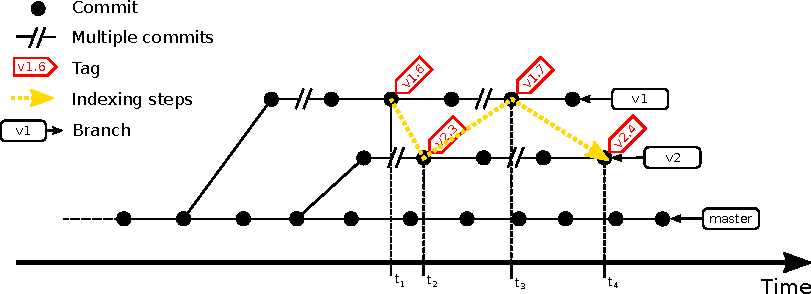
\includegraphics[width=\linewidth]{../written/figures/tag_sort.pdf}
\end{frame}

\begin{frame}
	Code Beispiele 
\end{frame}

\begin{frame}{Definition of infringement}
\begin{itemize}
	\item Study on Uniqueness of Code \cite{2010-gabel-su-source-code-uniqueness}:\\
	\textit{\enquote{general lack of uniqueness in [...] one to seven lines of source code}}
	\item Veritas Operating Corp. vs Microsoft Corp \cite{mertzel2008copying}:
	\textit{54 out of 160.000 lines of code copied}
\end{itemize}

\begin{center}
	\textbf{$\rightarrow$ 8 lines minimum, 54 critical}
\end{center}
Identical code fragments, excerpt whitespace and comments with changed, added or removed statements
\note{
	\begin{itemize}
		\item Kopie $\rightarrow$ Lizenzverletzung?
		\item Zwei Anhaltspunkte
		\item Trotzdem: abhängig inhalt
	\end{itemize}
}
\end{frame}

\end{document}